\chapter{Network simulation}

In order to evaluate network performance two main options were considered: using real IoT devices or using a network simulation tool.
Due to technical limitations that came with using real devices, such as not being able to access the router of our network, simulation was chosen.
In this chapter we will discuss how we used Mininet~\citep{lantz_mininet_2021}, a realistic virtual network, in our evaluation.

Mininet is a tool that can be used to created software-defined networks (SNDs) using the $OpenFlow$ standard.

\begin{figure}[ht]
    \centering
    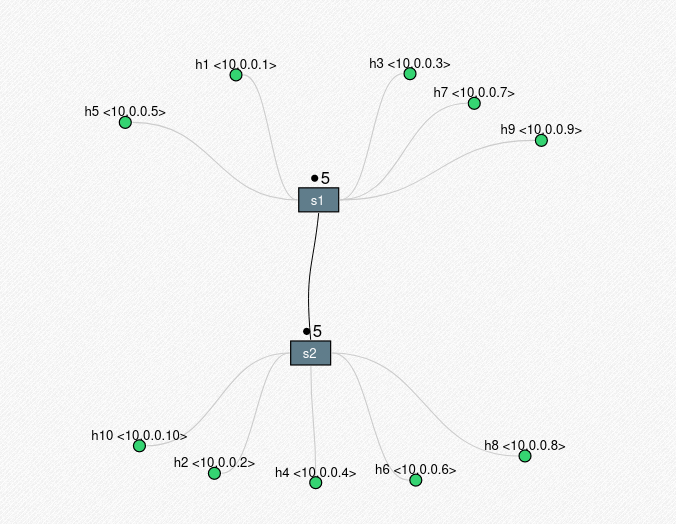
\includegraphics[width=0.5\linewidth]{images/mininet_topo.png}
    \caption{The resulting Dumbbell topology with 5 hosts on either side of the switch. This topology simulates congestion on the link as the hosts have to share it for their data transfer.}
    \label{fig:mininet-topo}
\end{figure}

Using the Python API provided we created the network topology shown in Figure~\ref{fig:mininet-topo}.
The script used takes several parameters in order to create a simulation environment resembling a realistic scenario.
The variables that the script changes between simulations to do so are the link's \textit{bandwidth}, \textit{delay} and the rate of \textit{packet loss}.

The bandwidth of a link is the maximum rate of data transfer we can achieve on it.
In contrast to bandwidth in signal processing, in computer networking bandwidth is typically measured in bits per second, rather than hertz.
The delay of a link specifies the latency in terms of the time that a bit of data has to travel across a link and is typically measured in milliseconds.
Link delay has a correspondence to the geographical distance between the communicating parties, however, in the case of IoT we can expect devices to be in local proximity.
Lastly, the rate of packet loss shows the percentage of packets that were corrupted or dropped in transit.
Due to these packets being retransmitted in various protocols, this rate also adds to the delay of data transfer.
Importantly, we have only considered the typical circumstances of packet loss and have not included scenarios such as interference or packet loss attacks.

The bandwidth and delay numbers correspond, as closely as possible, to various link types in a network.
To do so we have gathered data from the~\cite{ofcom_uk_2021} report on UK broadband speeds.
There were specific cases in which it was not possible to find this data in the report, hence it was augmented using a similar methodology in the work conducted by~\cite{previdi_is-is_2019} and in the case of ZigBee, the work by~\citet{alena_fault_2011}.

\begin{table}[ht]
    \caption{The parameters chosen for each link simulation in Mininet. The types of links were chosen as the most commonly occurring ones in IoT use cases. The data also assumes a typical IoT setup where most devices are within local geographical proximity. That is, the devices are communicating between each other within the range of one factory or site, with only the central node communicating with some server.}\label{tab:links}
    %\tt 
    \rowcolors{2}{}{gray!3}
    \begin{tabular}{@{}llll@{}}
        \toprule
        \textbf{Simulated Link Type} & \textbf{Link bandwidth (Mb/s)} & \textbf{Link delay (ms)} & \textbf{Packet loss rate (\%)} \\
        Wi-Fi                        & \texttt{30}                    & \texttt{10}              & \texttt{2}                     \\
        ZigBee                       & \texttt{0.25}                  & \texttt{5}               & \texttt{1}                     \\
        4G                           & \texttt{4}                     & \texttt{20}              & \texttt{1.5}                   \\
        3G                           & \texttt{1}                     & \texttt{40}              & \texttt{1.5}                   \\
        100Mb Ethernet               & \texttt{100}                   & \texttt{1}               & \texttt{0.2}                   \\
        \bottomrule
    \end{tabular}
\end{table}

It was especially difficult to find exact estimates for packet loss rates with most sources describing only what is a "good" rate for a stable connection~\citep{sdu_ictp-sdu_2013}.
Hence, the data are best estimates, cross-validated through the different sources and are not exact values.

Using the different links, a file of equal size was then transferred using the various QUIC implementations described in Chapter~\ref{chap:quic_impl}.